Los sistemas de organización del conocimiento, \textit{Knowledge Organization Systems} (\gls{KOS}), como
tesauros, taxonomías o sistemas de clasificación, se han desarrollado en el seno de distintas comunidades e instituciones, 
principalmente con el objetivo de organizar grandes bases de datos que contienen recursos de diferente tipo tales como documentos, 
páginas web o elementos multimedia. Estos vocabularios permiten a los usuarios la anotación
de los objetos de información de los recursos para simplificar su extracción y consulta, habitualmente 
se utilizan técnicas de indexado por un determinado tema con el objeto de facilitar el acceso también para las máquinas, 
suministrando los metadatos necesarios en la descripción de los objetos de información.

En el dominio de la contratación pública electrónica estas clasificaciones resultan de gran 
interés para la especificación de los objetos de contrato, así como para la extracción de 
estadísticas a posteriori. Como se ha reseñado en la Sección~\ref{sect:pscs}, una de las 
principales clasificaciones en este sentido es el ``\textit{Common Procurement Vocabulary}''(\gls{CPV})~\cite{cpvguide}, 
pero también existen otros esquemas de clasificación de gran interés en la esfera del comercio 
electrónico, así la ``\textit{Combined Nomenclature}'' o el ``\textit{North American Product Classification System}''. 
En el ámbito de esta tesis se ha optado por promocionar las clasificaciones más importantes en este contexto 
para facilitar el acceso a los anuncios de licitación independientemente de la clasificación utilizada, para ello, 
se ha realizado la transformación siguiendo los principios de \linkeddata y los métodos definidos en el capítulo anterior de 
las siguientes clasificaciones estándar de productos (\gls{PSC}s) (un total de $9$), ver Tabla~\ref{table:pscs-ld}.

\begin{longtable}[c]{|p{6cm}|l|p{6cm}|} 
\hline
  \textbf{Clasificación} &  \textbf{Acrónimo} & \textbf{Organismo} \\\hline
\endhead
\textit{Common Procurement Vocabulary}, (2003 y 2008) & \gls{CPV} & Unión Europea \\ \hline
\textit{Combined Nomenclature} 2012 (desde 1995) & \gls{CN} & Unión Europea  \\ \hline
\textit{Central Product Classification}, version 2 (2008) & \gls{CPC} & Unión Europea \\ \hline
Clasificación de Productos por Actividad (2008) & \gls{CPA} & Unión Europea \\ \hline
\textit{International Standard Industrial Classification of All Economic Activities, Rev.4} & \gls{ISIC} & \textit{United Nations Statistics Division} \\ \hline
\textit{North American Industry Classification System} 2007 y 2012 & \gls{NAICS} & Gobierno de Estados Unidos \\ \hline
\textit{Standard International Trade Classification, Revision 4} & \gls{SITC} & \textit{United Nations Statistics Division} \\ \hline
%\textit{Nomenclature générale des activités économiques dans les Communautés européennes} & NACE & Unión Europea \\ \hline
\hline
\caption{Catálogo de Clasificaciones Estándar de Productos seleccionadas.}\label{table:pscs-ld}\\    
\end{longtable}

\subsection{Proceso de Producción de \linkeddata de Clasificaciones\\ Estándar de Productos}
Siguiendo la definición realizada en la Sección~\ref{sect:produccion}, este proceso conlleva
todas las tareas que implican la transformación de un \dataset de entrada $\mathcal{G}$, mediante
unas reglas de \textit{mapeo} $\mathcal{M}$, para la obtención de un \dataset \gls{RDF} $\mathcal{D}$, método semántico 
de producción. 

\subsubsection{Tarea $t_1$-Análisis del \dataset a transformar}\label{t1-pscs}
Las \gls{PSC}s como instrumentos claves de estandarización nacen con el fin de
conseguir una clasificación común de productos y servicios. Las diferencias entre las clasificaciones no
sólo se limitan a cuestiones de alcance y cobertura sectorial de producto, sino también al grado de especificidad que difiere de unas a otras.

Como ya se ha reseñado en la Sección~\ref{semantica:pscs}, Hepp~\cite{HeppTrueComplexity,HeppEclass,HeppMethodology} apunta 
a estos estándares como una combinación de componentes variables que pueden ser utilizados 
para la construcción de ontologías derivadas, sin embargo, se puede identificar 
una estructura común subyacente a todas las PSCs y que debe considerarse fundamental para 
proporcionar un modelo de datos semántico universal para las PSCs, para ello, se utilizarán 
los conceptos los conceptos de \textit{árbol} y \textit{bosque} provenientes de la teoría de 
grafos con el objetivo de representar la estructura común de las PSCs. 

\begin{description}
 \item [Categorías de productos.] Las clasificaciones se dividen en categorías o
clases de productos. Estas categorías agrupan los distintos elementos de la PSC,
$Cat_{psc}$, en distintos niveles de especialización semántica o niveles de
jerarquía: $Cat_{psc} = \displaystyle\bigcup_{n=0}^k{(Cat_{psc}^n)}$, desde
términos genéricos, como el caso del elemento del \gls{CPV}-``Servicios de reparación y mantenimiento'' (código 50000000), hasta productos altamente
específicos y directamente identificables, como en un elemento de la misma jerarquía anterior pero con un mayor nivel 
de especificidad como ``Servicios de reparación y mantenimiento de instalaciones contra incendios'' (código 50413200). Una PSC cumple las siguientes
características:
\begin{itemize}
 \item Las categorías de la PSC se organizan jerárquicamente: $Cat_{psc}^0\succ
Cat_{psc}^1\succ...\succ Cat_{psc}^n $.
 \item Cada elemento de la PSC, $t_{psc}^x$, pertenece a una categoría de
productos.
 \item Cada elemento de la PSC, $t_{psc}^x$, pertenece sólo a una categoría de
productos. Es decir, las categorías son disjuntas:
$\displaystyle\bigcap_{n=0}^k{(Cat_{psc}^n)}=\emptyset$.
\end{itemize}


\item  [Estructura taxonómica.] Además de la división en niveles de jerarquía
de los elementos de una \gls{PSC}, su objetivo es organizar y agrupar los productos en
sectores verticales mediante algún tipo de criterio establecido por la comunidad
que desarrolla el estándar. Formalmente, esta estructura taxonómica de cada
sector de productos tiene forma de árbol, $T_{psc}$: todos los elementos
$t_{psc}^n$ tienen un elemento de nivel superior $t_{psc}^{n-1}$. Además el
conjunto de sectores de productos de una clasificación constituye la propia PSC,
que puede definirse como un \textbf{bosque} ($\mathbb{F}_{psc}$) de árboles
($T_{psc}$), en el que se cumple que:
\begin{itemize}
 \item $\mathbb{F}_{psc}= \displaystyle\bigcup_{m=0}^k{(T_{psc}^m)}$
 \item Cada elemento $t_{psc}^0$ es la \textbf{raíz} de una agrupación de
productos estructurada jerárquicamente en forma de árbol, $T_{psc}^x$.
 \item Cada elemento $t_{psc}$ pertenece a uno de estos árboles de productos
$T_{psc}^x$.
 \item Por la propia definición de bosque, cada elemento $t_{psc}$ pertenece sólo
a un $T_{psc}^x$. Es decir, cada sector de productos es disjunto:
$\displaystyle\bigcap_{m=0}^k{(T_{psc}^m)}=\emptyset$.
\end{itemize}
 
\end{description}

Estas son características genéricas de las clasificaciones de productos, sin
embargo, otras PSCs más sofisticadas incluyen un diccionario de propiedades
estándar que se puede utilizar para describir productos con más detalle.
Normalmente, estos diccionarios de propiedades también incluyen los tipos de
datos que pueden ser valor de las mismas, así como su referencia con respecto
a estándares internacionales para establecer las unidades de medida, tal es el caso
de la clasificación de productos de e@Class. En otras ocasiones, se construyen
clasificaciones multiling\"{u}es para la expresión de los descriptores de cada
elemento de la PSC, el caso extremo es el \gls{CPV}, donde se contempla un total de hasta $23$ lenguas.

El desafío básico más importante que hay que afrontar cuando se deriva una
ontología de una PSC, reside en cómo interpretar la semántica original de la taxonomía.
No existe una definición formal de las relaciones taxonómicas que construyen
cada $T_{psc}$ de la clasificación y es tentador utilizar la propiedad de un
vocabulario de ontologías, como \textit{rdfs:subClassOf}, para intentar
representar estas relaciones semánticas. La postura del enfoque seguido es 
radicalmente distinta, ver Sección~\ref{semantica:pscs}, desde este punto de vista, las PSCs fueron construidas 
para solucionar problemas de comunicación, proporcionar una
forma de organizar tipos de productos y agruparlos de acuerdo a unos conceptos y
definiciones que funcionasen \textit{de facto} como un estándar en determinados
entornos de actividad comercial e industrial. Las PSCs no fueron diseñadas como
modelos conceptuales de dominio, en el sentido actual que tiene el término
``ontología'', sino como una forma de estructurar la terminología y la forma de
nombrar los productos, de ahí que se interpreten las PSCs como simples
esquemas conceptuales en el que la relación taxonómica que jerarquiza los
distintos elementos de cada $T_{psc}$ no se interpreta como una relación de
herencia o subtipo, sino como una relación de mayor o menor especificidad de los
elementos. Resumiendo, se consideran las PSCs como simples vocabularios
controlados y se utilizará una ontología RDF/\gls{OWL}, \gls{SKOS} Core, como modelo de
datos común.

La adopción de una ontología como SKOS Core para modelar las PSCs está
completamente justificada desde este enfoque, se trata de una ontología RDF/OWL que gira en torno a dos clases principales
\textit{skos:Concept} y \textit{skos:ConceptScheme}, así todos los elementos de una
PSC son considerados instancias de \textit{skos:Concept}, de manera que se
entiende que todos ellos son conceptualizaciones de recursos. Asumiendo este
modelo, la interpretación de cada elemento $t_{psc}$ de una PSC es natural, directa y no provoca incoherencias en su 
tratamiento, tal como se ha reseñado en los ejemplos anteriores de inconsistencia. El interés de este enfoque, radica en la posibilidad de poder 
replicar completamente la semántica original de las PSCs.

Para agrupar todos los elementos de una \gls{PSC} bajo un paraguas común, se construye una
clase contenedora de todos los $t_{psc}$: $PSCConcept$, declarándola como
subclase del concepto $skos:Concept$: 

\begin{equation}
 PSCConcept \sqsubseteq skos:Concept
\end{equation}

Esta clase a su vez se puede dividir en distintas categorías que constituyen
los niveles de jerarquía del PSC (si los hubiera). El atractivo en la utilización de SKOS Core reside 
en que es factible replicar completamente el modelo de datos común de las PSCs, de esta forma, por cada $Cat_{psc}^k$,
se construye un concepto subclase de \textit{PSCConcept}, en el caso particular del \gls{CPV}:

\begin{equation}
 Division \sqsubseteq PCSConcept;Grupo \text{...}
\end{equation}

Y se mantiene la semántica original de la clasificación añadiendo los siguientes
axiomas, perfectamente expresables en OWL-DL para el caso del CPV. En otras clasificaciones, no 
es posible establecer este tipo de axiomas debido a la falta de designación de categorías ya que la 
relación de jerarquía se establece simplemente mediante un código numérico.

\begin{equation}
 PSCConcept\ \equiv Division\ \sqcup\ Grupo \sqcup\ Clase\ \sqcup\ Categoria
\end{equation}

\begin{equation}
Division \sqcap\ Grupo \sqcap\ Clase\ \sqcap\ Categoria = \perp
\end{equation}

Por otro lado, el segundo factor importante a destacar reside en la estructura taxonómica de cada
$T_{psc}$, que como se ha referido, tenía una difícil interpretación como conjunto de
relaciones de herencia clásica, sin embargo, bajo el paradigma SKOS Core se contemplan relaciones 
semánticas tales como: \texttt{skos:inScheme}, \texttt{skos:related}, \texttt{skos:broader}, \texttt{skos:narrower} y sus versiones transitivas, que
constituyen el marco conceptual adecuado para el establecimiento de las relaciones entre los elementos de la PSC.

Finalmente, la clase \textit{skos:ConceptScheme} deviene necesario para completar la 
interpretación de una PSC y su modelo, ver Figura~\ref{fig:modelo-grafico-pscs}, se reifica 
una PSC como una instancia de esta clase para también así contextualizar los 
términos y distinguirlos e identificarlos en lo referido a un entorno web.

\begin{equation}
 PSCConcept \equiv\ni inScheme~PSCScheme
\end{equation}


\begin{figure}[!htp]
 \centering
	 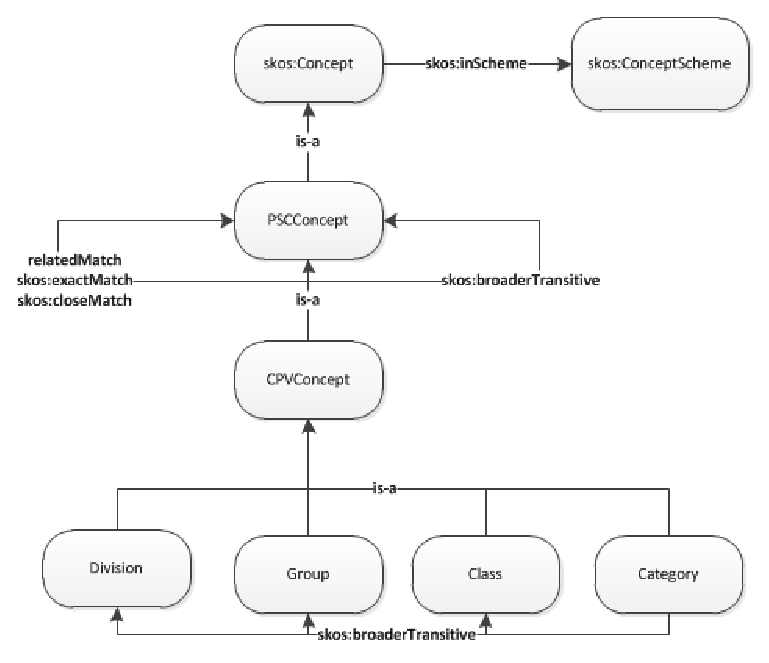
\includegraphics[width=10cm]{images/phd/modelo/pscs-model}
	\caption{Modelo gráfico para las Clasificaciones Estándar de Productos.}
	\label{fig:modelo-grafico-pscs}
\end{figure}



\subsubsection{Tarea $t_2$-Limpieza de datos}
Los datos provenientes de las clasificaciones de productos se encuentran disponibles, en la mayoría de los casos, 
en hojas de cálculo MSExcel o bien directamente en formato \gls{CSV} en los cuales ya se ha realizado un esfuerzo por los organismos 
creadores para evitar caracteres extraños o incorrectos. Habitualmente, todos estos datos provienen de fuentes oficiales por lo que
este proceso ya ha sido realizado en la labor de creación de los mismos, es por lo que en la promoción de estos datos, esta tarea
ya ha sido realizada y no es necesario aplicar ningún filtro especial a los datos ya disponibles. Esta circunstancia supone 
un gran avance para la transformación de datos, ya que se dispone de aquellos clasificados con $2\star$ según los principios de \linkeddata y no 
es necesario realizar procesos de \textit{screen-scrapping} con la consiguiente ganancia en la calidad de los datos.

\subsubsection{Tarea $t_3$-Selección de Vocabularios}
Los vocabularios seleccionados para modelar las clasificaciones de productos, teniendo en cuenta el análisis 
realizado en la tarea $t_1$ se presentan en la Tabla~\ref{table:pscs-select-vocabs}. En general, se trata de vocabularios 
que atienden a los siguientes criterios:

\begin{enumerate}
 \item Formalización de una estructura taxonómica, como RDFS, \gls{SKOS} u \gls{OWL}.
 \item Realización de \textit{mapeos} entre conceptos, como SKOS y OWL.
 \item Representación de tipos de datos, como \gls{XML Schema}.
 \item Gestión de información multiling\"{u}e, como \gls{SKOS-XL} y RDFS.
 \item Representación de información de negocio, como \textit{GoodRelations} y \textit{ProductOntology}.
 \item Adición de metadatos y \textit{provenance}, como \textit{Dublin Core Terms}, \gls{voID} y \textit{Provenance Ontology}.
 \item Representación del tiempo e intervalos, como \textit{Time Ontology} del \gls{W3C}.
\end{enumerate}


\begin{longtable}[c]{|l|p{4cm}|p{4cm}|p{4cm}|} 
\hline
\textbf{Prefijo} &  \textbf{Vocabulario} &  \textbf{Fuente} & \textbf{Uso} \\\hline
\endhead
 dbpedia & \url{http://dbpedia.org/ontology/}&  Comunidad \linkeddata. & Reutilización de definiciones. \\ \hline 
 dc & \url{http://purl.org/dc/elements/1.1/}&  \textit{Dublin Core Metadata Initiative} & Creación de metadatos para los documentos. \\ \hline  
 dct & \url{http://dublincore.org/documents/dcmi-terms/}&  $\equiv$ & $\equiv$ \\ \hline  
 foaf & \url{http://xmlns.com/foaf/0.1/} &Comunidad de Web Semántica.& Especificación de relaciones entre personas. \\ \hline 
 gr & \url{http://purl.org/goodrelations/v1#} & Martin Heep & Reutilización de definiciones para describir productos y servicios.\\\hline 
 owl  & \url{http://www.w3.org/2002/07/owl#} & W3C & Realización de definiciones en el dominio. \\\hline
 po & \url{http://www.productontology.org/} & \textit{Martin Heep} & Reutilización de datos provenientes de Productontology.\\\hline 
 skos & \url{http://www.w3.org/2004/02/skos/core#} & W3C & Especificación de taxonomías. \\ \hline
 skosxl & \url{http://www.w3.org/2008/05/skos-xl#>} & W3C & Representación de información ling\"uística. \\ \hline
 rdf & \url{http://www.w3.org/1999/02/22-rdf-syntax-ns#} & W3C & Descripción de recursos. \\ \hline
 rdfs & \url{http://www.w3.org/2000/01/rdf-schema#} & W3C & Descripción de recursos con relaciones lógicas. \\ \hline 
 void & \url{http://rdfs.org/ns/void#} & Deri y W3C & Descripción de metadatos de un \dataset. \\\hline
 xml & \url{http://www.w3.org/XML/1998/namespace} & W3C & Reutilización de definiciones. \\\hline
 xsd & \url{http://www.w3.org/2001/XMLSchema#} & W3C & Especificación de tipos de datos. \\\hline
\hline
\caption{Selección de Vocabularios para las Clasificaciones Estándar de Productos.}\label{table:pscs-select-vocabs}\\    
\end{longtable}

\subsubsection{Tarea $t_4$-Selección de otros \datasets RDF}
Al igual que en la sección anterior, los \datasets a reutilizar se centran en vocabularios de negocio 
ya existentes y por consiguiente en los datos disponibles en los mismos, de esta forma, se reutilizan 
y enlazan datos provenientes de \textit{GoodRelations} y \textit{ProductOntology}, ver Tabla~\ref{table:pscs-select-datasets}.

\begin{longtable}[c]{|l|p{4cm}|p{4cm}|p{4cm}|} 
\hline
  \textbf{Prefijo} &  \textbf{\textit{Dataset}} &  \textbf{Fuente} & \textbf{Uso} \\\hline
\endhead
dbpedia-res & \url{http://dbpedia.org/}&  Comunidad \linkeddata. & Reutilización de datos provenientes de la DBPedia. \\ \hline 
gr & \url{http://purl.org/goodrelations/v1#} & \textit{Martin Heep} & Reutilización de definiciones para describir productos y servicios.\\\hline 
po & \url{http://www.productontology.org/} & \textit{Martin Heep} & Reutilización de datos provenientes de ProductOntology.\\\hline 
\hline
\caption{Selección de otros \datasets para las Clasificaciones Estándar de Productos.}\label{table:pscs-select-datasets}\\    
\end{longtable}


\subsubsection{Tarea $t_5$-Modelado de datos en RDF}\label{sect:pscs-data-model}
El resultado de esta tarea debe ser una ontología de dominio $\mathcal{O}$. que modele los recursos $t_{psc}$, pertenecientes a un 
\dataset RDF $\mathcal{D}$. Inicialmente, se debe proveer la especificación del modelo 
formal u ontología $\mathcal{O}$ de acuerdo al análisis realizado en la Sección~\ref{t1-pscs}, dando soporte 
a la descripción de los datos de los recursos \gls{RDF}:

\begin{itemize}
 \item $\mathcal{C} = \{$\textit{PSCConcept, CPVConcept, Division, Group, Class, Category}$\}$
 \item $\mathcal{R} = \{$\textit{rdf:type, skos:inScheme, dc:identifier, dc:subject, level, pscs:relatedMatch, pscs:level, skos:exactMatch, skos:broaderTransitive, skos:prefLabel, rdfs:label, gr:description}$\}$
 \item $\mathcal{I} = \{ t_{psc} \}$
 \item $\mathcal{A} = \{\star\}$, son los axiomas propios de una ontología en SKOS.
\end{itemize}
 
Como segundo paso se diseñan las propiedades que deben tener los recursos, teniendo en cuenta su ulterior aplicación, 
ver Tabla~\ref{table:pscs-rdf-model}, pertenecientes a ese \dataset, comunes para todas las \gls{PSC}s.

Una vez especificado el conjunto de propiedades de cada elemento $t_{psc}$ es necesario definir el conjunto 
de grafos en los cuales se encuadrarán los recursos, es decir, el \dataset \gls{RDF} $\mathcal{D}$. Para ello, 
en la Tabla~\ref{table:pscs-dataset} se indican las tuplas $(\mathcal{G}_k, I_k)$ correspondientes a cada uno 
de los grafos $\mathcal{G}_k$ identificados a través de la URI $I_k$.

\begin{longtable}[c]{|p{3cm}|p{9cm}|} 
\hline
  \textbf{$\mathcal{G}_k$} &  \textbf{$I_k$}  \\\hline
\endhead
 \textbf{$\mathcal{G}$}   & \url{http://purl.org/weso/pscs} \\ \hline
 \textbf{$\mathcal{G}_1$} & \url{http://purl.org/weso/pscs/cpv/2008} \\ \hline
 \textbf{$\mathcal{G}_2$} & \url{http://purl.org/weso/pscs/cpv/2003} \\ \hline
 \textbf{$\mathcal{G}_3$} & \url{http://purl.org/weso/pscs/cn/2012} \\ \hline
 \textbf{$\mathcal{G}_4$} & \url{http://purl.org/weso/pscs/cpc/2008} \\ \hline
 \textbf{$\mathcal{G}_5$} & \url{http://purl.org/weso/pscs/cpa/2008} \\ \hline
 \textbf{$\mathcal{G}_6$} & \url{http://purl.org/weso/pscs/isic/v4} \\ \hline
 \textbf{$\mathcal{G}_7$} & \url{http://purl.org/weso/pscs/naics/2007} \\ \hline
 \textbf{$\mathcal{G}_8$} & \url{http://purl.org/weso/pscs/naics/2012} \\ \hline
 \textbf{$\mathcal{G}_9$} & \url{http://purl.org/weso/pscs/sitc/v4} \\ \hline
 \textbf{$\mathcal{G}_{10}$} & \url{http://purl.org/weso/pscs/ontology} \\ \hline 
\hline
\caption{\textit{Dataset} RDF $\mathcal{D}$ para Clasificaciones Estándar de Productos.}\label{table:pscs-dataset}\\    
\end{longtable}


\begin{longtable}[c]{|p{5cm}|p{4.5cm}|p{5cm}|} 
\hline
  \textbf{Propiedad} &  \textbf{Descripción} & \textbf{Ejemplo} \\\hline
  \texttt{rdf:type} & Especificación del tipo de un recurso $t_{psc}$ & a \texttt{gr:ProductOr ServiceModel}, \texttt{PSCConcept} \\ \hline
  \texttt{skos:inScheme} & \gls{URI} al esquema de la PSC $T_{psc}$ a la que pertenece $t_{psc}$ & \texttt{skos:inScheme} cpv2008:ds \\ \hline
  \texttt{dc:identifier} & Identificador utilizado en la URI del recurso $t_{psc}$ &  \texttt{dc:identifier} "55900000"$\textasciicircum\textasciicircum$xsd:string \\ \hline
  \texttt{dc:subject} & Identificador original proveniente de la fuente de datos &  \texttt{dc:subject} "55900000-9"$\textasciicircum\textasciicircum$xsd:string \\ \hline
  \texttt{pscs:relatedMatch} & URI a un recurso $t'_{psc}$ que encaja parcialmente con $t_{psc}$ & \texttt{po:retail} \\ \hline
  \texttt{skos:exactMatch } & URI a un recurso $t'_{psc}$ que encaja totalmente con $t_{psc}$ & \texttt{cpv2008:52900000} \\ \hline
  \texttt{skos:closeMatch } & URI a un recurso $t'_{psc}$ del CPV 2008 que encaja parcialmente con $t_{psc}$ & \texttt{cpv2008:52900000} \\ \hline
  \texttt{pscs:level} & Indica el grado de especificidad de un $t_{psc}$ cuando no se puede inferir directamente su antecesor & \texttt{pscs:level} ``5'' \\ \hline  
  \texttt{skos:broaderTransitive} & URI a un recurso $t'_{psc}$ antecesor de $t_{psc}$ que indica la categoría $Cat_{psc}$ & \texttt{skos:broaderTransitive} cpv2008:55000000 \\ \hline
  \texttt{skos:prefLabel} & Etiquetas y descripciones multing\"{u}es &  "Retail trade services"@EN \\ \hline
  \texttt{rdfs:label} & $\equiv$ &  $\equiv$\\ \hline
  \texttt{gr:description} & $\equiv$ &  $\equiv$ \\ \hline
\endhead
\hline
\caption{Diseño de propiedades para los elementos de las Clasificaciones Estándar de Productos.}\label{table:pscs-rdf-model}\\    
\end{longtable}




\subsubsection{Tarea $t_6$-Diseño de un Esquema de URIs}
Esta tarea tiene como objetivo establecer la forma y estructura de las \gls{URI}s tanto para las definiciones 
realizadas en la ontología $\mathcal{O}$ como para todos los recursos presentes en el \dataset RDF $\mathcal{D}$ que 
se genera a partir de la transformación de los datos a \gls{RDF}. Es una de las actividades clave ya que guiará 
tanto el método final de transformación como el proceso posterior de publicación. En la Tabla~\ref{table:pscs-uris} se 
hace la descripción de la estructura de URIs que se seguirán para las \gls{PSC}s.

\begin{longtable}[c]{|p{5cm}|p{4.5cm}|p{5cm}|} 
\hline
  \textbf{URI} &  \textbf{Descripción} & \textbf{Ejemplo} \\\hline
\endhead
\url{http://purl.org/weso/pscs/} & URI base: <base\_uri> & NA \\ \hline
\url{<base_uri>/ontology} & Definiciones comunes a todas las PSC & \url{<base_uri>/ontology/PSCConcept} \\ \hline
\url{<base_uri>/resource/ds} & Descripción del catálogo de las PSCs & \url{<base_uri>/resource/ds} \\ \hline
\url{<base_uri>/{psc}/{version|year}} & Espacio de nombres para una determinada PSC & \url{<base_uri>/cpv/2008} \\ \hline
\url{<base_uri>/{psc}/{version|year}/ontology} & Definiciones particulares de una PSC & \url{<base_uri>/cpv/2008/ontology} \\ \hline
\url{<base_uri>/resource/{psc}/{version|year}/{id}} & URI para un recurso de una PSC & \url{<base_uri>/cpv/2008/resource/55900000} \\ \hline
\url{<base_uri>/resource/{psc}/{version|year}/ds} & URI la descripción del \dataset de una PSC & \url{<base_uri>/cpv/2008/resource/ds} \\ \hline
\hline
\caption{Diseño de URIs para las Clasificaciones Estándar de Productos.}\label{table:pscs-uris}\\    
\end{longtable}

\subsubsection{Tarea $t_7$-Diseño Plantilla Objetivo del Recurso RDF}
El objetivo de esta tarea es establecer una plantilla de cada uno de los recursos RDF que están 
presentes en el \dataset \gls{RDF} $\mathcal{D}$ para que sirvan como guía en los siguientes momentos: 1) en la ejecución propiamente dicha 
de la transformación de los datos originales a RDF y 2) en la validación de los recursos RDF generados. De esta manera, 
tratándose de \datasets con una gran cantidad de recursos se pueden identificar fácilmente aquellos que no sean 
compatibles con este esquema favoreciendo la depuración de los recursos generados. Adicionalmente, un esquema de 
recurso sirve como documentación extra para el proceso de consumo. En el caso de las clasificaciones de productos es necesario 
establecer un recurso plantilla, ver Figura~\ref{fig:pscs-template}, para los propios elementos de la \gls{PSC}, $t_{psc}$, así como para la propia descripción 
de los \datasets. No obstante, esta descripción se delega a la tarea $t_{16}$-``Añadir metainformación a los recursos RDF'', 
ver Sección~\ref{t16-pscs}.

De acuerdo al recurso plantilla y a las definiciones realizadas en la ontología que modela estos datos 
es posible realizar una validación en cuanto a los tipos de datos, cardinalidad de las relaciones, tipo de objetos, etc., que 
resulta de sumo interés para asegurar la calidad de los datos producidos.

\begin{figure}[!htp]
\begin{lstlisting} 
<<base_uri>/resource/{psc}/{version|year}/{id}>
      a       gr:ProductOrServiceModel , pscs:PSCConcept;
     (skos:prefLabel ""@lang;)+
     (gr:description ""@lang;)+
     (rdfs:label ""@lang ;)+
     dc:identifier ""^^xsd:string ;
     dc:subject ""^^xsd:string ;
     (pscs:relatedMatch <uri>;)*
     (pscs:level <uri>;)*
     (skos:broaderTransitive <uri>;)[0,1]
     (skos:exactMatch <uri>; )*
     skos:inScheme <<base_uri>/resource/{psc}/{version|year}/ds> .	
\end{lstlisting}
	\caption{Plantilla Objetivo de un Recurso de las Clasificaciones Estándar de Productos.}
	\label{fig:pscs-template}
\end{figure}



\subsubsection{Tarea $t_8$-Enriquecimiento de los datos en RDF}\label{t8-pscs}
El objetivo de esta tarea es enlazar los recursos generados del \dataset RDF $\mathcal{D}$ con otros 
ya existentes. En el caso particular de las clasificaciones de productos y de acuerdo a los \datasets 
identificados en la Tarea $t_4$, el enriquecimiento de los elementos se realizará con \textit{ProductOntology} que 
a su vez dispone de enlaces a la DBPedia, con lo que el enlazado de los datos queda perfectamente justificado. 

Para llevar a cabo el enriquecimiento es necesario realizar reconciliación de entidades entre las descripciones 
de elementos $t_{psc}$ y los recursos objetivos. Análogamente a enfoques como los de \textit{Silk Server} o SERIMI y teniendo 
en cuenta las particularidades de las descripciones de los productos se ha decido implementar un componente, 
como parte de \texttt{moldeas-transformer}, para realizar este enlazado, tomando como entrada la descripción del producto, en inglés, y tras 
la realización del procesamiento de lenguaje natural mediante las herramientas Apache \gls{Lucene}~\cite{Hatcher:2004:LA:1044938} y \gls{Solr}~\cite{solr}, obtiene una lista de recursos 
candidatos a ser enlazados. Dado que el \textit{matching} de los recursos no se puede asegurar al 100\%, requeriría una validación manual, 
por lo que se ha creado una propiedad particular \textit{pscs:relatedMatch} para indicar la relación que se establece entre el recurso 
actual $t_{psc}$ y el recurso obtenido. Adicionalmente, en una segunda versión se ha especializado esta propiedad para incluir 
un valor de fiabilidad (\textit{threshold}) que indica el grado de similitud entre los recursos, de esta manera se pueden obtener 
los recursos similares a uno dado por encima de un valor umbral.

Por otra parte, en el ámbito de los anuncios de licitación la clasificación de productos más relevante es el \gls{CPV} 2008 ya que 
es el sistema de clasificación vigente y normativo en la Unión Europea. Teniendo en cuenta que los anuncios de licitación 
objeto de estudio en este documento pertenecen a la Unión Europea y que por lo tanto están clasificados de acuerdo a esta 
taxonomía, es conveniente proveer los enlaces adecuados entre los distintos elementos de todas las PSCs para que puedan 
ser traducidos al CPV 2008 facilitando la capacidad expresiva para la realización de consultas y en consecuencia favoreciendo 
la accesibilidad a los anuncios de licitación. El soporte a este enfoque sigue un modelo similar al presentado anteriormente, 
con la diferencia de que los recursos origen son aquellos generados en la transformación de las \gls{PSC}s y el \dataset objetivo 
es el correspondiente al CPV 2008. De esta manera, se establecen dos tipos de enlaces:
\begin{enumerate}
 \item \textit{Mapping} exacto. Este enlace entre elementos de las PSCs se realiza cuando en las propias clasificaciones existen 
\textit{mapeos} entre los elementos porque un organismo oficial se ha encargado de realizar esta tarea por cuestiones estratégicas. En este caso, 
el enlace entre los conceptos se modela mediante la propiedad \texttt{skos:exactMatch} cuya semántica dentro de la especificación 
de SKOS indica que su uso estará destinado a realizar enlaces entre conceptos \textit{skos:Concept}, en los cuales se puede asegurar 
que representan al mismo recurso.
\item \textit{Mapping} parcial. Al igual que en el caso anterior el proceso consiste en identificar los recursos del CPV 2008 que encajan 
parcialmente con un recurso origen en otra PSC. En este caso, la propiedad utilizada es \texttt{skos:closeMatch} que de acuerdo 
a su semántica permite establecer enlaces entre conceptos \textit{skos:Concept}. Igualmente, se ha especializado este caso 
para contener un valor umbral del enlace.
\end{enumerate}
 
En conclusión, la ejecución de esta tarea permite por un lado crear enlaces entre todas las PSCs y un \dataset externo y por otra parte, 
crear enlaces entre todas las PSCs y el CPV 2008. El enriquecimiento realizado en las PSCs conduce finalmente a la siguiente estructura, 
ver Figura~\ref{fig:linked-pscs}, de enlaces entre las distintas PSCs y los \datasets externos.

\begin{figure}[!htb]
\centering
	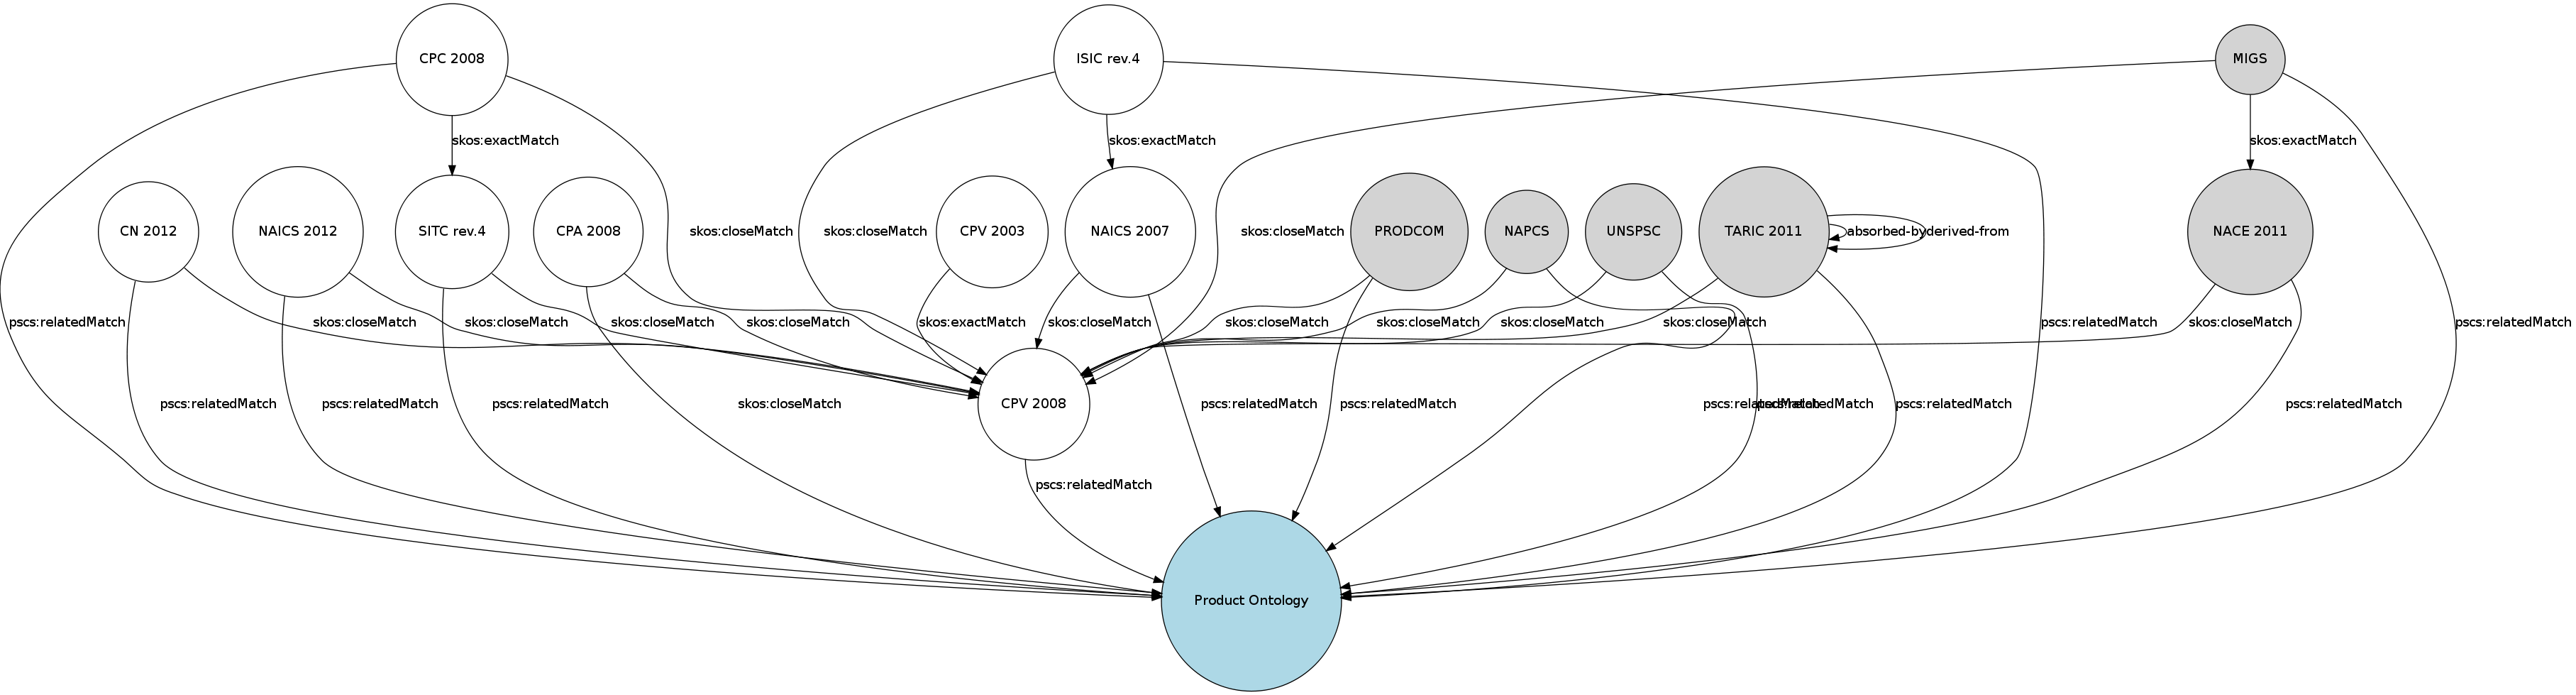
\includegraphics[width=20cm,angle=90]{./images/phd/pscs}
\caption{Enlaces entre las distintas Clasificaciones de Productos.}
\label{fig:linked-pscs}
\end{figure}

\subsubsection{Tarea $t_9$-Transformación de los datos a RDF }
Una vez realizadas las tareas anteriores se está en disposición de realizar la transformación 
de los datos de entrada a \gls{RDF}. En esta tarea el punto clave de decisión reside en seleccionar bien 
una herramienta ya disponible o bien implementar un programa que ejecute las reglas de transformación 
tomando como entrada los datos de las clasificaciones. En el caso objeto de estudio se ha optado 
por un enfoque híbrido realizando la transformación inicial mediante la herramienta Google Refine~\cite{google-refine} y su extensión~\cite{grefine} 
para trabajar con RDF y las posteriores etapas de enriquecimiento a través de una implementación particular que tenga en cuenta 
la casuística específica de las clasificaciones de productos. En cualquier caso, en la ejecución de esta 
tarea se debe asegurar que el \dataset RDF $\mathcal{D}$ generado es válido en cuanto a sintaxis y al modelo definido. Esta tarea 
se ha ejecutado secuencialmente para cada unas de las clasificaciones de productos.
% 
% \begin{figure}[!htb]
% \centering
% 	%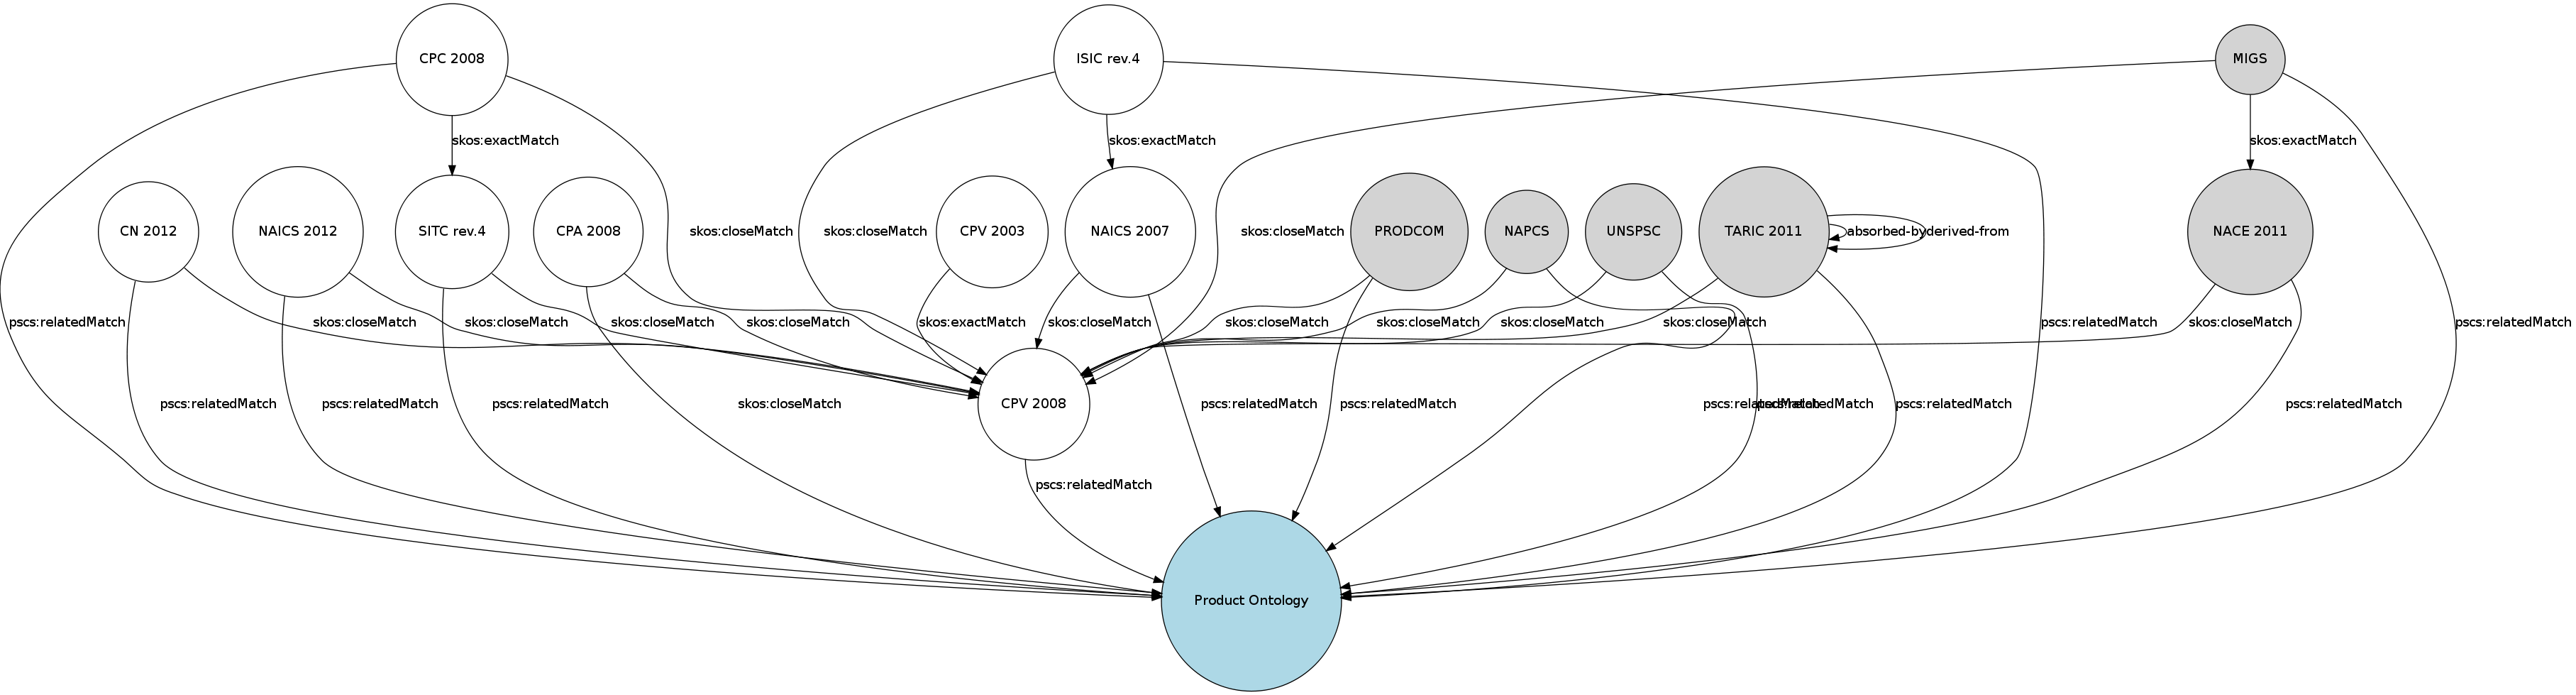
\includegraphics[width=18cm,angle=90]{./images/phd/pscs}
% \caption{Tarea $t_9$-Transformación de los Datos a RDF de las Clasificaciones de Productos.}
% \label{fig:t9-pscs}
% \end{figure}

\subsubsection{Tarea $t_{10}$-Reconciliación de Entidades}
El diseño y ejecución de esta tarea ha sido descrito en la Sección~\ref{t8-pscs} ya que están 
estrechamente ligadas.

\subsubsection{Tarea $t_{16}$-Añadir metainformación a los recursos RDF}\label{t16-pscs}
En el caso de las clasificaciones de productos la metainformación en los recursos se puede 
interpretar en los dos sentidos que se han descrito en la Sección~\ref{t16-metodos}, bien 
en cada uno de los recursos generados o en el \dataset completo. Considerando el carácter 
estático de las clasificaciones de productos en cuanto a su creación, depende de los organismos oficiales que 
se encargan de su mantenimiento, y dado que para los elementos que varían en el tiempo éstos 
generan un \textit{mapeo} directo entre las versiones de los mismos, como en el caso del CPV 2003 y 2008, se considera 
una elección correcta situar la metainformación a nivel de \dataset para cada unas de las PSCs. Para ello y de acuerdo 
a los vocabularios seleccionados se utiliza \textit{\gls{voID}} como especificación para indicar la metainformación 
de un \dataset concreto. El enfoque seguido genera metainformación a nivel del catálogo de las clasificaciones 
de producto, ver Figura~\ref{fig:pscs-ls}, y para cada una de las clasificaciones transformadas, ver Figura~\ref{fig:pscs-ds-cpv-2008} como ejemplo 
de la descripción del \dataset del \gls{CPV} 2008. Es relevante destacar la definición de la licencia de los datos con el objetivo 
de facilitar su posterior reutilización, en este caso se ha optado por una licencia de ``\textit{Open Data}'' basada en las directrices 
fijadas en la guía provista en~\cite{od-license}.

\begin{figure}[!htp]
\begin{lstlisting} 
<http://purl.org/weso/pscs/data/resource/ds?output=ttl>
      rdfs:label "RDF description of Product Scheme Classifications" ;
      foaf:primaryTopic <http://purl.org/weso/pscs/resource/ds> .

<http://purl.org/weso/pscs/resource/ds>
      a    <http://rdfs.org/ns/void#Linkset> ;
      rdfs:label "Product Scheme Classifications"@en ;
      dcterms:author 
            <http://www.di.uniovi.es/~labra/labraFoaf.rdf#me> , 
	    <http://www.josemalvarez.es/foaf.rdf#me> ;
      dcterms:contributor
            <http://purl.org/weso/pscs/resource/10ders> ,
	    <http://rdfohloh.wikier.org/project/moldeas/rdf> ;
      dcterms:description 
            "Some Product Scheme Classifications available in RDF" ;
      dcterms:license
            <http://opendatacommons.org/licenses/by/1.0/> ;
      dcterms:modified
            "2011-11-10"^^<http://www.w3.org/2001/XMLSchema#date> ;
      dcterms:publisher
            <http://www.josemalvarez.es/foaf.rdf#me> ;
       dcterms:title
            "Product Scheme Classifications" ;
      void:target
            <http://purl.org/weso/pscs/cpc/2008/resource/ds> , 
	    <http://purl.org/weso/pscs/naics/2007/resource/ds> , 
	    <http://purl.org/weso/pscs/sitc/v4/resource/ds> , 
	    <http://purl.org/weso/pscs/cpv/2003/resource/ds> , 
	    <http://purl.org/weso/pscs/naics/2012/resource/ds> , 
	    <http://purl.org/weso/pscs/cpv/2008/resource/ds> , 
	    <http://purl.org/weso/pscs/cpa/2008/resource/ds> , 
	    <http://purl.org/weso/pscs/cn/2012/resource/ds> , 
	    <http://purl.org/weso/pscs/isic/v4/resource/ds> ;
      foaf:homepage <http://purl.org/weso> .	
\end{lstlisting}
	\caption{Descripción del \textit{Linkset} de las Clasificaciones Estándar de Productos.}
	\label{fig:pscs-ls}
\end{figure}


\begin{figure}[!htp]
\begin{lstlisting} 
<http://purl.org/weso/pscs/cpv/2008/resource/ds>
      a       void:Dataset , skos:ConceptScheme ;
      rdfs:label "CPV 2008"@en ;
      dcterms:author 
            <http://www.di.uniovi.es/~labra/labraFoaf.rdf#me> , 
	    <http://www.josemalvarez.es/foaf.rdf#me> ;
      dcterms:contributor
            <http://purl.org/weso/pscs/resource/10ders> ,
	    <http://rdfohloh.wikier.org/project/moldeas/rdf> ;
      dcterms:description "Common Procurement Vocabulary" ;
      dcterms:license <http://opendatacommons.org/licenses/by/1.0/> ;
      dcterms:modified "2011-11-10"^^xsd:date ;
      dcterms:publisher <http://www.josemalvarez.es/foaf.rdf#me> ;
      dcterms:source 
	<http://europa.eu/legislation_summaries/internal_market/businesses/public_procurement/l22008_en.htm> ;
      dcterms:title "CPV 2008" ;
      void:dataDump <http://purl.org/weso/pscs/cpv/2008/cpv-2008.ttl> ;
      void:exampleResource
        <http://purl.org/weso/pscs/cpv/2008/resource/18000000> , 
	<http://purl.org/weso/pscs/cpv/2008/resource/45000000> , 
	<http://purl.org/weso/pscs/cpv/2008/resource/33000000> ;
      void:uriRegexPattern
        "http://purl.org/weso/pscs/cpv/2008/resource/.+" ;
      void:vocabulary dc: , skos: , gr: ;
      skos:hasTopConcept 
	<http://purl.org/weso/pscs/cpv/2008/resource/63000000> ,
	<http://purl.org/weso/pscs/cpv/2008/resource/76000000> , 
	<http://purl.org/weso/pscs/cpv/2008/resource/19000000> , 
	<http://purl.org/weso/pscs/cpv/2008/resource/79000000> , 	
	...
	<http://purl.org/weso/pscs/cpv/2008/resource/16000000> ;
      foaf:homepage <http://purl.org/weso> .
\end{lstlisting}
	\caption{Descripción del \dataset CPV 2008.}
	\label{fig:pscs-ds-cpv-2008}
\end{figure}
\clearpage
\subsubsection{Resultado Final y Ejemplos}\label{resultado-pscs}
El resultado final del proceso de producción de \linkeddata, tras el análisis y ejecución 
de las tareas identificadas y del método de producción seleccionado, genera como resultado un catálogo 
de clasificaciones de productos mediante datos enlazados, en los cuales se pueden extraer las siguientes 
estadísticas de producción de datos así como ejemplos de los recursos generados, ver Tabla~\ref{table:pscs-ejemplos}. Por otra parte, 
el aumento de la expresividad en el momento de realizar consultas se puede observar en la Figura~\ref{fig:pscs-sparql-query} en la 
que se expresa la siguiente consulta:

\begin{Frame}
\textit{``Dame 100 productos o servicios relacionados, descripción en inglés, con el término construcción que aparezca en cualquiera de los catálogos disponibles y 
que tengan enlaces con productos o servicios disponibles en la CPV 2008.''}
\end{Frame}


\begin{longtable}[c]{|p{2.5cm}|p{2.5cm}|p{1.8cm}|p{1.8cm}|p{2.5cm}|p{2.5cm}|} 
\hline
  \textbf{Clasificación} & \textbf{Nº de Elementos}  &  \textbf{Ejemplo} &  \textbf{Tripletas} &  \textbf{Enlaces externos} &  \textbf{Enlaces CPV 2008} \\\hline
\endhead
\gls{CPV} 2003 & $8323$  & Figura~\ref{fig:pscs-example-cpv-2003}   & $546135$  & $8322$ & $462$ (del CPV 2008 al 2003)   \\ \hline
CPV 2008 & $10357$ &  Figura~\ref{fig:pscs-example-cpv-2008}   & $803311$  & $10355$ & N/A   \\ \hline
\gls{CN} 2012  & $14552$& Figura~\ref{fig:pscs-example-cn-2012}      & $137484$  & $2590$ & $2390$ \\ \hline
\gls{CPC} 2008 & $4408$&  Figura~\ref{fig:pscs-example-cpc-2008}    & $100819$  & $4408$ & $4375$ y $1503$ (exactos)  \\ \hline
\gls{CPA} 2008 & $5429$&  Figura~\ref{fig:pscs-example-cpa-2008}    & $92749$   & $5429$ & $5399$  \\ \hline
\gls{ISIC} v4  & $766$& Figura~\ref{fig:pscs-example-isic-rev4}    & $18986$   & $766$ & $765$  \\ \hline
\gls{NAICS} 2007 & $2328$& Figura~\ref{fig:pscs-example-naics-2007} & $36292$   & $2328$ & $2300$  \\ \hline
NAICS 2012 & $2212$& Figura~\ref{fig:pscs-example-naics-2012} & $35390$   & $2212$ & $2186$  \\ \hline
\gls{SITC} v4 & $4017$&  Figura~\ref{fig:pscs-example-sitc-v4}      & $70887$   & $3941$ & $3811$  \\ \hline
\multicolumn{6}{|c|}{\textbf{Catálogo de Clasificaciones Estándar de Productos} (total)} \\ \hline
PSCs & $52392$ &  N/A & $1842053$ & $40351$ & $23191$  \\ \hline
\hline
\caption{Estadísticas y Ejemplos del Catálogo de Clasificaciones Estándar de Productos seleccionadas.}\label{table:pscs-ejemplos}\\    
\end{longtable}

\begin{figure}[!htp]
\begin{lstlisting} 
SELECT DISTINCT * WHERE{
  ?product pscs:relatedMatch <http://www.productontology.org/id/construction> .
  ?product skos:closeMatch ?cpv.
  ?product skos:prefLabel ?productLabel.
  ?cpv skos:prefLabel ?cpvLabel.
  ?product skos:inScheme ?scheme.
  FILTER (?scheme != <http://purl.org/weso/pscs/cpv/2008/resource/ds>).
  FILTER (lang(?cpvLabel)="en")
} LIMIT 100
\end{lstlisting}
	\caption{Ejemplo de consulta en SPARQL sobre el Catálogo de Clasificaciones de Productos.}
	\label{fig:pscs-sparql-query}
\end{figure}

\begin{figure}[!htp]
\lstinputlisting{examples/e-proc/cpv-2003.ttl}
	\caption{Ejemplo final de un Recurso del CPV 2003.}
	\label{fig:pscs-example-cpv-2003}
\end{figure}

\begin{figure}[!htp]
	\lstinputlisting{examples/e-proc/cpv-2008.ttl}
	\caption{Ejemplo final de un Recurso del CPV 2008.}
	\label{fig:pscs-example-cpv-2008}
\end{figure}

\begin{figure}[!htp]
\lstinputlisting{examples/e-proc/cn-2012.ttl}
	\caption{Ejemplo final de un Recurso de CN 2012.}
	\label{fig:pscs-example-cn-2012}
\end{figure}

\begin{figure}[!htp]
\lstinputlisting{examples/e-proc/cpc-2008.ttl}
	\caption{Ejemplo final de un Recurso de CPC 2008.}
	\label{fig:pscs-example-cpc-2008}
\end{figure}


\begin{figure}[!htp]
\lstinputlisting{examples/e-proc/cpa-2008.ttl}
	\caption{Ejemplo final de un Recurso de CPA 2008.}
	\label{fig:pscs-example-cpa-2008}
\end{figure}


\begin{figure}[!htp]
\lstinputlisting{examples/e-proc/isic-v4.ttl}
	\caption{Ejemplo final de un Recurso de ISIC rev4.}
	\label{fig:pscs-example-isic-rev4}
\end{figure}


\begin{figure}[!htp]
\lstinputlisting{examples/e-proc/naics-2007.ttl}
	\caption{Ejemplo final de un Recurso de NAICS 2007.}
	\label{fig:pscs-example-naics-2007}
\end{figure}


\begin{figure}[!htp]
\lstinputlisting{examples/e-proc/naics-2012.ttl}
	\caption{Ejemplo final de un Recurso de NAICS 2012.}
	\label{fig:pscs-example-naics-2012}
\end{figure}


\begin{figure}[!htp]
\lstinputlisting{examples/e-proc/sitc-v4.ttl}
	\caption{Ejemplo final de un Recurso de SITC v4.}
	\label{fig:pscs-example-sitc-v4}
\end{figure}


\clearpage
\subsubsection{Método de Producción de \linkeddata de Clasificaciones Estándar de Productos}
De acuerdo al análisis y diseño de datos enlazados realizado para las clasificaciones de productos 
a lo largo de las anteriores anteriores y la tabla de decisión~\ref{tabla:produccion}, el método semántico seleccionado 
para realizar la producción de datos enlazados es el $SPM_1$-``Transformación de datos a RDF'', ver Sección~\ref{spm-1}, en el 
se transforman un conjunto de datos de entrada $\mathcal{G}$ a un \dataset \gls{RDF} $\mathcal{D}$. Según la definición de método 
semántico de producción, realizada en la Sección~\ref{method-prod-def}, y el estudio de las clasificaciones de productos se pueden 
establecer los siguientes conjuntos:
\begin{itemize}
 \item $\mathcal{G}$ es el \dataset de entrada, conjunto de tuplas, conteniendo los datos de cada una de las clasificaciones de productos.
 \item $\mathcal{M}$ es el conjunto de \textit{mapeos}, ver Tabla~\ref{table:pscs-mappings}, extraídos según el análisis y diseño realizado en las secciones anteriores. Estos 
\textit{mapeos} son directamente expresables en la herramienta de transformación y toman como parámetros el valor de una de las tuplas de entrada (posición $X$) y la propiedad a generar.
 \item \textit{Dataset} RDF $\mathcal{D}$ es el \dataset resultado, siguiendo el análisis y diseño realizado en las secciones anteriores y tras la ejecución 
de la tarea propia de transformación de datos.
\end{itemize}

\begin{longtable}[c]{|p{2cm}|p{8cm}|p{4cm}|} 
\hline
  \textbf{$\mathcal{M}$} &  \textbf{Propiedad} & \textbf{Valor} \\\hline
\endhead
 $m_1$ & \texttt{rdf:type} & \gls{URI} \\ \hline
 $m_2$ & \texttt{skos:inScheme} & URI  \\ \hline
 $m_3$ & \texttt{dc:identifier} & \texttt{xsd:string} \\ \hline
 $m_4$ & \texttt{dc:subject} & \texttt{xsd:string} \\ \hline
 $m_5$ & \texttt{pscs:relatedMatch} & URI  \\ \hline
 $m_6$ & \texttt{skos:exactMatch } & URI \\ \hline
 $m_7$ & \texttt{skos:closeMatch } & URI  \\ \hline
 $m_8$ & \texttt{pscs:level} & \texttt{xds:int} \\ \hline  
 $m_9$ & \texttt{skos:broaderTransitive} & URI \\ \hline
 $m_{10}$ & \texttt{skos:prefLabel}, \texttt{rdfs:label}, \texttt{gr:description}  & \texttt{xsd:string@lang} \\ \hline   
\hline
\caption{Conjunto de \textit{mapeos} $\mathcal{M}$ para las Clasificaciones Estándar de Productos.}\label{table:pscs-mappings}\\    
\end{longtable}

\subsection{Proceso de Publicación de \linkeddata de Clasificaciones\\ Estándar de Productos}\label{sect:proceso-publicacion-ld}
Considerando que la estrategia definida para todos los \datasets implicados en el proceso de contratación pública 
electrónica es común, el proceso de publicación es homogéneo siguiendo la estructura definida 
en la Sección~\ref{sect:proceso-publicacion-ld}.

\newpage

\subsubsection{Tarea $t_{14}$-Infraestructura para \linkeddata}
Nuevamente, la estrategia definida para todos los \datasets implicados en el proceso de contratación pública 
electrónica es común, por ello la infraestructura utilizada es la misma que la definida 
en la Sección~\ref{infraestructura-comun}.

\subsubsection{Tarea $t_{15}$-Acceso y formato en datos RDF}
De la misma forma que en el apartado anterior, el acceso y formato de datos RDF para los datos contenidos y relativos 
a las organizaciones siguen el esquema proporcionado en la Sección~\ref{t15-comun}.

\subsection{Proceso de Consumo de Clasificaciones Estándar\\ de Productos}
El proceso de consumo de datos enlazados, según la definición realizada en la Sección~\ref{sect:proceso-consumo}, consiste en 
la reutilización de los datos enlazados para ser aplicados en la construcción de una nueva aplicación o servicio de valor 
añadido. En general, la reutilización más sencilla consiste en la representación gráfica de los recursos o la simple 
consulta con selección de formato de datos de acuerdo a las características de publicación utilizadas. En el caso 
que nos ocupa y teniendo en cuenta el objetivo de realización de un prototipo experimental de extracción de anuncios 
de licitación como demostrador del consumo de datos enlazados, se ha escogido el método semántico de consumo $SCM_2$-``\textit{Mapeo} a Lenguaje de Programación'', 
cuya descripción está disponible en la Sección~\ref{scm2-consumo}, orientado a obtener una representación de los recursos RDF en un 
lenguaje de programación (en este caso Java) como objetos de negocio. De acuerdo a este objetivo y la definición del propio método 
es necesario definir:
\begin{itemize}
 \item El \dataset RDF $\mathcal{D}_{pub}$, es el conjunto de datos disponible tras aplicar el método de publicación.
 \item El conjunto $\mathcal{M}^1$, ver Tabla~\ref{table:pscs-consumo}, indica como transformar el \dataset anterior a la representación objetivo, objetos del lenguaje Java.
\end{itemize}

De esta manera, se obtiene una serie de objetos, $\mathcal{D}_{consum}$, con la información y datos necesarios, no se transforman necesariamente todos los datos disponibles en los recursos pertenecientes 
a  $\mathcal{D}_{pub}$, para ser reutilizados como objetos de negocio en un lenguaje de programación. Es conveniente señalar que el acceso a los datos se realiza a través 
de la consulta al \textit{endpoint} de \gls{SPARQL} ejecutando consultas \textit{SELECT} y \textit{DESCRIBE}.

\begin{longtable}[c]{|p{2cm}|p{6cm}|p{6cm}|} 
\hline
  \textbf{$\mathcal{M}^1$} &  \textbf{Propiedad} & \textbf{Tipo en Java} \\\hline
\endhead
 $m^1_1$ & URI recurso     		& \texttt{java.lang.String} \\ \hline
 $m^1_2$ & \texttt{rdf:type}      	& \texttt{org.weso.moldeas.to.PSCTO} \\ \hline
 $m^1_3$ & \texttt{skos:inScheme} 	& \texttt{java.lang.String}  \\ \hline
 $m^1_4$ & \texttt{dc:identifier} 	& \texttt{java.lang.String} \\ \hline
 $m^1_5$ & \texttt{dc:subject}    	& \texttt{java.lang.String} \\ \hline
 $m^1_6$ & \texttt{pscs:relatedMatch} 	& \texttt{java.util.List<PSCTO> } \\ \hline
 $m^1_7$ & \texttt{skos:exactMatch } 	& \texttt{java.util.List<PSCTO> }\\ \hline
 $m^1_8$ & \texttt{skos:closeMatch } 	& \texttt{java.util.List<PSCTO>}  \\ \hline
 $m^1_9$ & \texttt{pscs:level} 	& int \\ \hline  
 $m^1_{10}$ & \texttt{skos:broaderTransitive} & java.util.List<PSCTO>  \\ \hline
 $m^1_{11}$ & \texttt{skos:prefLabel}, \texttt{rdfs:label}, \texttt{gr:description}  & Map<String,String> (lang, value) para cada propiedad \\ \hline   

\hline
\caption{Conjunto de \textit{mapeos} $\mathcal{M}^1$ de consumo para las Clasificaciones Estándar de Productos.}\label{table:pscs-consumo}\\    
\end{longtable}

\subsection{Proceso de Validación de Clasificaciones Estándar de Productos}
La validación como proceso transversal en cualquier etapa dentro del ciclo de vida de datos 
enlazados debe realizarse con el objetivo de asegurar la calidad de los datos. De acuerdo a la 
definición realizada en la Sección~\ref{sect:validation}, este proceso consiste en la comprobación 
de que los recursos de un \dataset RDF cumplen ciertas características. 

La realización de esta validación puede ser realizada manual o automáticamente en función del caso concreto, por ejemplo para la característica 
de negociación de contenido o para la inclusión en la nube de datos enlazados se dispone de herramientas adecuadas, pero 
en cambio para comprobaciones relativas a los dominios y rangos de las propiedades, etc., no existe una 
herramienta completa. Por todo ello, se ha seguido un enfoque híbrido basado en la utilización de herramientas 
y validación manual. La descripción completa de la validación de acuerdo a todas las características 
se reseña en las Tablas de Validación disponibles en el Apéndice~\ref{tablas-validacion-apen}.

\subsubsection{Tarea $t_{12}$-Validación de Recursos RDF}
Siguiendo con la definición realizada de esta tarea en la Sección~\ref{lod-t12}, se puede asegurar que la transformación 
realizada de los catálogos de clasificaciones de productos a la iniciativa \linkeddata cumple estrictamente los 
siguientes puntos:

\begin{itemize}
 \item Los datos \gls{RDF} son correctos ya que se han utilizado herramientas y \gls{API}s (Google \gls{Refine} y Jena) que aseguran 
la generación correcta de RDF.
 \item El dominio y rango en las propiedades es correcta, ya que se realiza la validación contra el modelo definido.
 \item Se ha establecido metainformación sobre la procedencia a nivel de \dataset.
 \item Todos los recursos transformados siguen la plantilla objetivo RDF.
\end{itemize}

\subsection{Proceso de Realimentación de Clasificaciones\\ Estándar de Productos}
Este proceso según la definición realizada en la Sección~\ref{proceso-realimentacion}, busca la mejora 
y perfeccionamiento de los datos promocionados a \gls{RDF}. Esta situación emerge en el momento en el cual 
los datos comienzan a ser reutilizados, tanto por aplicaciones o servicios como por individuos. En el caso 
particular del catálogo de las clasificaciones de productos y debido a su reutilización por la 
\textit{Charles University} de la República Checa se han detectado errores que han sido 
corregidos, se trata de casos específicos no detectados por el proceso de validación, debido al procesamiento masivo de datos. 
En este sentido el proceso de realimentación se basa en un enfoque en el cual \textit{Usuarios y Aplicaciones} realizan 
el descubrimiento de datos no correctos y cuyo cambio se centra en una \textit{Actualización Ocasional}. Aunque 
este enfoque es completamente válido, es conveniente señalar que este proceso todavía no se ha definido de forma 
completa dentro de la iniciativa de \linkeddata por lo que su ejecución automática constituye un objetivo 
a medio plazo en el que terceros puedan mejorar los datos previa validación del \textit{Propietario de datos}.